\subsection{DNA Cloning}
The transformation with the new constructs was validated by sequencing following the mini-preparation. All clones showed 100\% sequence identity with the designs. The concentrations of the plasmids after the midi preparation were measured as \SI{605}{\nano\gram\per\micro\litre} (d29-A), \SI{335}{\nano\gram\per\micro\litre} (S-Tag-A), and \SI{300}{\nano\gram\per\micro\litre} (S-Tag-B), corresponding to yields of \SI{302}{\micro\gram}, \SI{167}{\micro\gram}, and \SI{150}{\micro\gram}.

\subsection{Protein Analysis}
\subsubsection{eYFP Yield by Fluorescence}
For an estimate of the protein yield in the cell-free expression mix, a fluorescence analysis of a cell-free expression setup expressing Strep-eYFP was conducted. The calibration showed a linear trend with a coefficient of determination of $R^2 = 0.98$ (\autoref{fig:calibration_eyfp}). Applying the linear model to the sample values, the concentration of Strep-eYFP in the reaction mixture was estimated as \SI{295}{\micro\gram\per\milli\litre}.

\subsubsection{Coomassie Staining and Western Blot} 
Coomassie staining and Western Blot were conducted both directly after the cell-free expression and after the following CaptoCore purification. For each setting, two blots were developed, one using an anti-PVX antibody, and one using an anti-S-Tag antibody. 

For the samples from cell-free expression (\autoref{fig:blot_alice}), the Coomassie Staining shows a wide range of bands. For the samples from ALiCE setups expressing d29-A, S-Tag-A, and S-Tag-B, the pattern looks very similar to that of the non-template control. The sample expressing Strep-eYFP has a notable band at a height corresponding to ~\SI{30}{\kilo\Dalton}, similar to the single band in the Strep-eYFP control. The track containing the S-Tag-CP-PVX control also displays a single band at ~\SI{29}{\kilo\Dalton}, slightly lower than that of the Strep-eYFP control. The sample from the ALiCE setup expressing PVX CP presents a band ~\SI{29}{\kilo\Dalton} as well. 

In the Western Blot based on the anti-PVX antibody, the samples from the ALiCE expressions of d29-A, S-Tag-A, and PVX CP show strong bands at ~\SI{25}{\kilo\Dalton}, ~\SI{31}{\kilo\Dalton}, and ~\SI{29}{\kilo\Dalton}. The band for the expressed PVX CP is particularly strong. The sample from S-Tag-B shows a faint band at ~\SI{28}{\kilo\Dalton}. The control S-Tag-CP-PVX has two bands visible in the blot, a stronger band at ~\SI{28}{\kilo\Dalton}, and a less prominent one at ~\SI{30}{\kilo\Dalton}. In all samples, the observed bands migrated to higher molecular weights than the theoretical molecular weights of \SI{22.6}{\kilo\Dalton} (d29-A), \SI{26.9}{\kilo\Dalton} (S-Tag-A), \SI{26.8}{\kilo\Dalton} (S-Tag-B), \SI{25.1}{\kilo\Dalton} (PVX CP), and \SI{26.9}{\kilo\Dalton} (S-Tag-CP-PVX).

In the blot using the anti-S-Tag antibody, the tracks containing samples from the expression of S-Tag-A and S-Tag-B show a strong signal. For S-Tag-A, the blot shows strong lines at ~\SI{31}{\kilo\Dalton}, ~\SI{29}{\kilo\Dalton}, and ~\SI{28}{\kilo\Dalton}, but with a fainter, diffuse trail to higher and lower molecular weights. In the track containing S-Tag-B, there are prominent lines visible at molecular weights of ~\SI{29}{\kilo\Dalton}, ~\SI{28}{\kilo\Dalton}, and ~\SI{25}{\kilo\Dalton}, as well as a faint, diffuse trail similar to that of S-Tag-A. The control containing S-Tag-CP-PVX shows a strong band at ~\SI{32}{\kilo\Dalton} and a faint band at ~\SI{30}{\kilo\Dalton}.

The Western Blot following the CaptoCore purification at first showed faint signals in the tracks for S-Tag-A for both the anti-PVX and the anti-S-Tag antibody, in the track for PVX CP using the anti-PVX antibody (\autoref{fig:blot_capto}). However, the samples of the purification showed some white precipitate, possibly resin from the column. Due to this, both the chromatography and Western Blot were repeated. In this second iteration, the samples from the column appeared clear and neither the Coomassie Gel nor the Western Blot showed signals (\autoref{fig:blot_capto_repetition}). No control was used in the second iteration.


\begin{figure}
\includegraphics{lab/blot_alice.png}
\caption{\textbf{Coomassie Gel and Western Blot images following ALiCE expression.} Samples were taken from the cell-free reaction mix of the constructs d29-A (S1), S-Tag-A (S2), S-Tag-B (S3), PVX CP (S4), Strep-eYFP (S5), and the non-template (S6). The controls used were purified Strep-eYFP (C1), and S-Tag-PVX virions (C2). The marker was NEB Color Prestained Protein Standard, Broad Range (10-250 kDa). In the Western Blot, the anti-PVX antibody creates signals for samples from d29-A, S-Tag-A, PVX CP, the control S-Tag-PVX, and a faint signal for S-Tag-B. The anti-S-Tag antibody leads to signals for S-Tag-A, S-Tag-B, and S-Tag-PVX. }
\label{fig:blot_alice}
\end{figure}

\begin{figure}
\includegraphics{lab/blot_capto_repetition.png}
\caption{\textbf{Coomassie Gel and Western Blot images following CaptoCore Purification.} Samples were taken from the concentrated CaptoCore flow-through for the constructs d29-A (S1), S-Tag-A (S2), S-Tag-B (S3), and PVX CP (S4). No control was used in the experiment. The marker was NEB Color Prestained Protein Standard, Broad Range (10-250 kDa). The blot created no signal for any of the samples. }
\label{fig:blot_capto_repetition}
\end{figure}


\label{subsection:elisa}
\subsubsection{ELISA}
For a quantitative analysis of the cell-free protein expression, an ELISA was performed on the samples, using both the anti-PVX antibody, and the anti-S-Tag antibody. 

The calibration measurements for the anti-PVX antibody show saturation at protein concentrations larger than \SI{100}{\nano\gram\per\milli\litre}. The four calibration samples below that threshold follow a linear trend 
\begin{equation}
\text{OD} = \SI{6.5}{\micro\litre\per\nano\gram} \cdot c
\end{equation}
with a coefficient of determination of $R^2=0.90$ (\autoref{fig:elisa_calib}). The measurements from the samples yielded significant OD values for d29-A, S-Tag-A, and PVX CP, and no significant signal for S-Tag-B and the non-template H\textsuperscript{2}O from the ALiCE expressions (\autoref{tab:sample_values_elisa_anti_pvx}). For d29-A, S-Tag-A, and PVX CP, the measured ODs of the different dilutions were almost identical, with an OD of ~0.2 for d29-A, 0.22 for S-Tag-A, and ~0.87 for PVX CP. Therefore, the back-calculated concentrations for the original undiluted sample vary over the two dilutions. Calculations based on the stronger diluted samples result in concentrations of \SI{30\pm 5}{\micro\gram\per\milli\litre} for d29-A, \SI{33\pm 4}{\micro\gram\per\milli\litre} for S-Tag-A, and \SI{134\pm 4}{\micro\gram\per\milli\litre} for PVX CP. 

For the anti-S-Tag antibody, calibration was sub-linear for low concentrations, but followed a linear trend for the whole sample range up to \SI{1500}{\nano\gram\per\milli\litre}. The linear model was calculated as 
\begin{equation}
\text{OD} = \SI{0.9}{\micro\litre\per\nano\gram} \cdot c
\end{equation}
and yielded a coefficient of determination of $R^2 = 0.98$ (\autoref{fig:elisa_calib}). As for the anti-PVX antibody, the sample OD measurements were highly similar for the 1:500 and 1:1000 dilutions (\autoref{tab:sample_values_elisa_anti_s_tag}), with significant ODs of 2.4/2.2 (1:500/1:1000)  for S-Tag-A and 1.5/1.1 (1:500/1:1000) for S-Tag-B. The samples of d29-A, PVX CP, and the non-template control showed no significant absorbtion. Following back-calculation of the stronger dilution, the concentration for S-Tag-A was evaluated as \SI{2400\pm 90}{\micro\gram\per\milli\litre}, and for S-Tag-B as \SI{1200\pm 100}{\micro\gram\per\milli\litre}.

\subsubsection{Electron Microscopy}
For clarification whether the constructs were able to form particles, the purified samples from the constructs d29-A, S-Tag-A, S-Tag-B, PVX CP, and a control of S-Tag-CP-PVX particles expressed in plants were analyzed using transmission electron microscopy. The construct S-Tag-A and the cell-free expressed PVX CP showed some clumped, darker areas that are also present in the non-template control (\autoref{em_overview}). The TEM images for d29-A showed little to no larger structures. For the control of S-Tag-PVX virions, a network of flexible filamentous rod-shaped particles was visible, with diameters of approximately \SI{17}{\nano\meter} and lengths of approximately \SI{600}{\nano\meter}. 

\begin{figure}
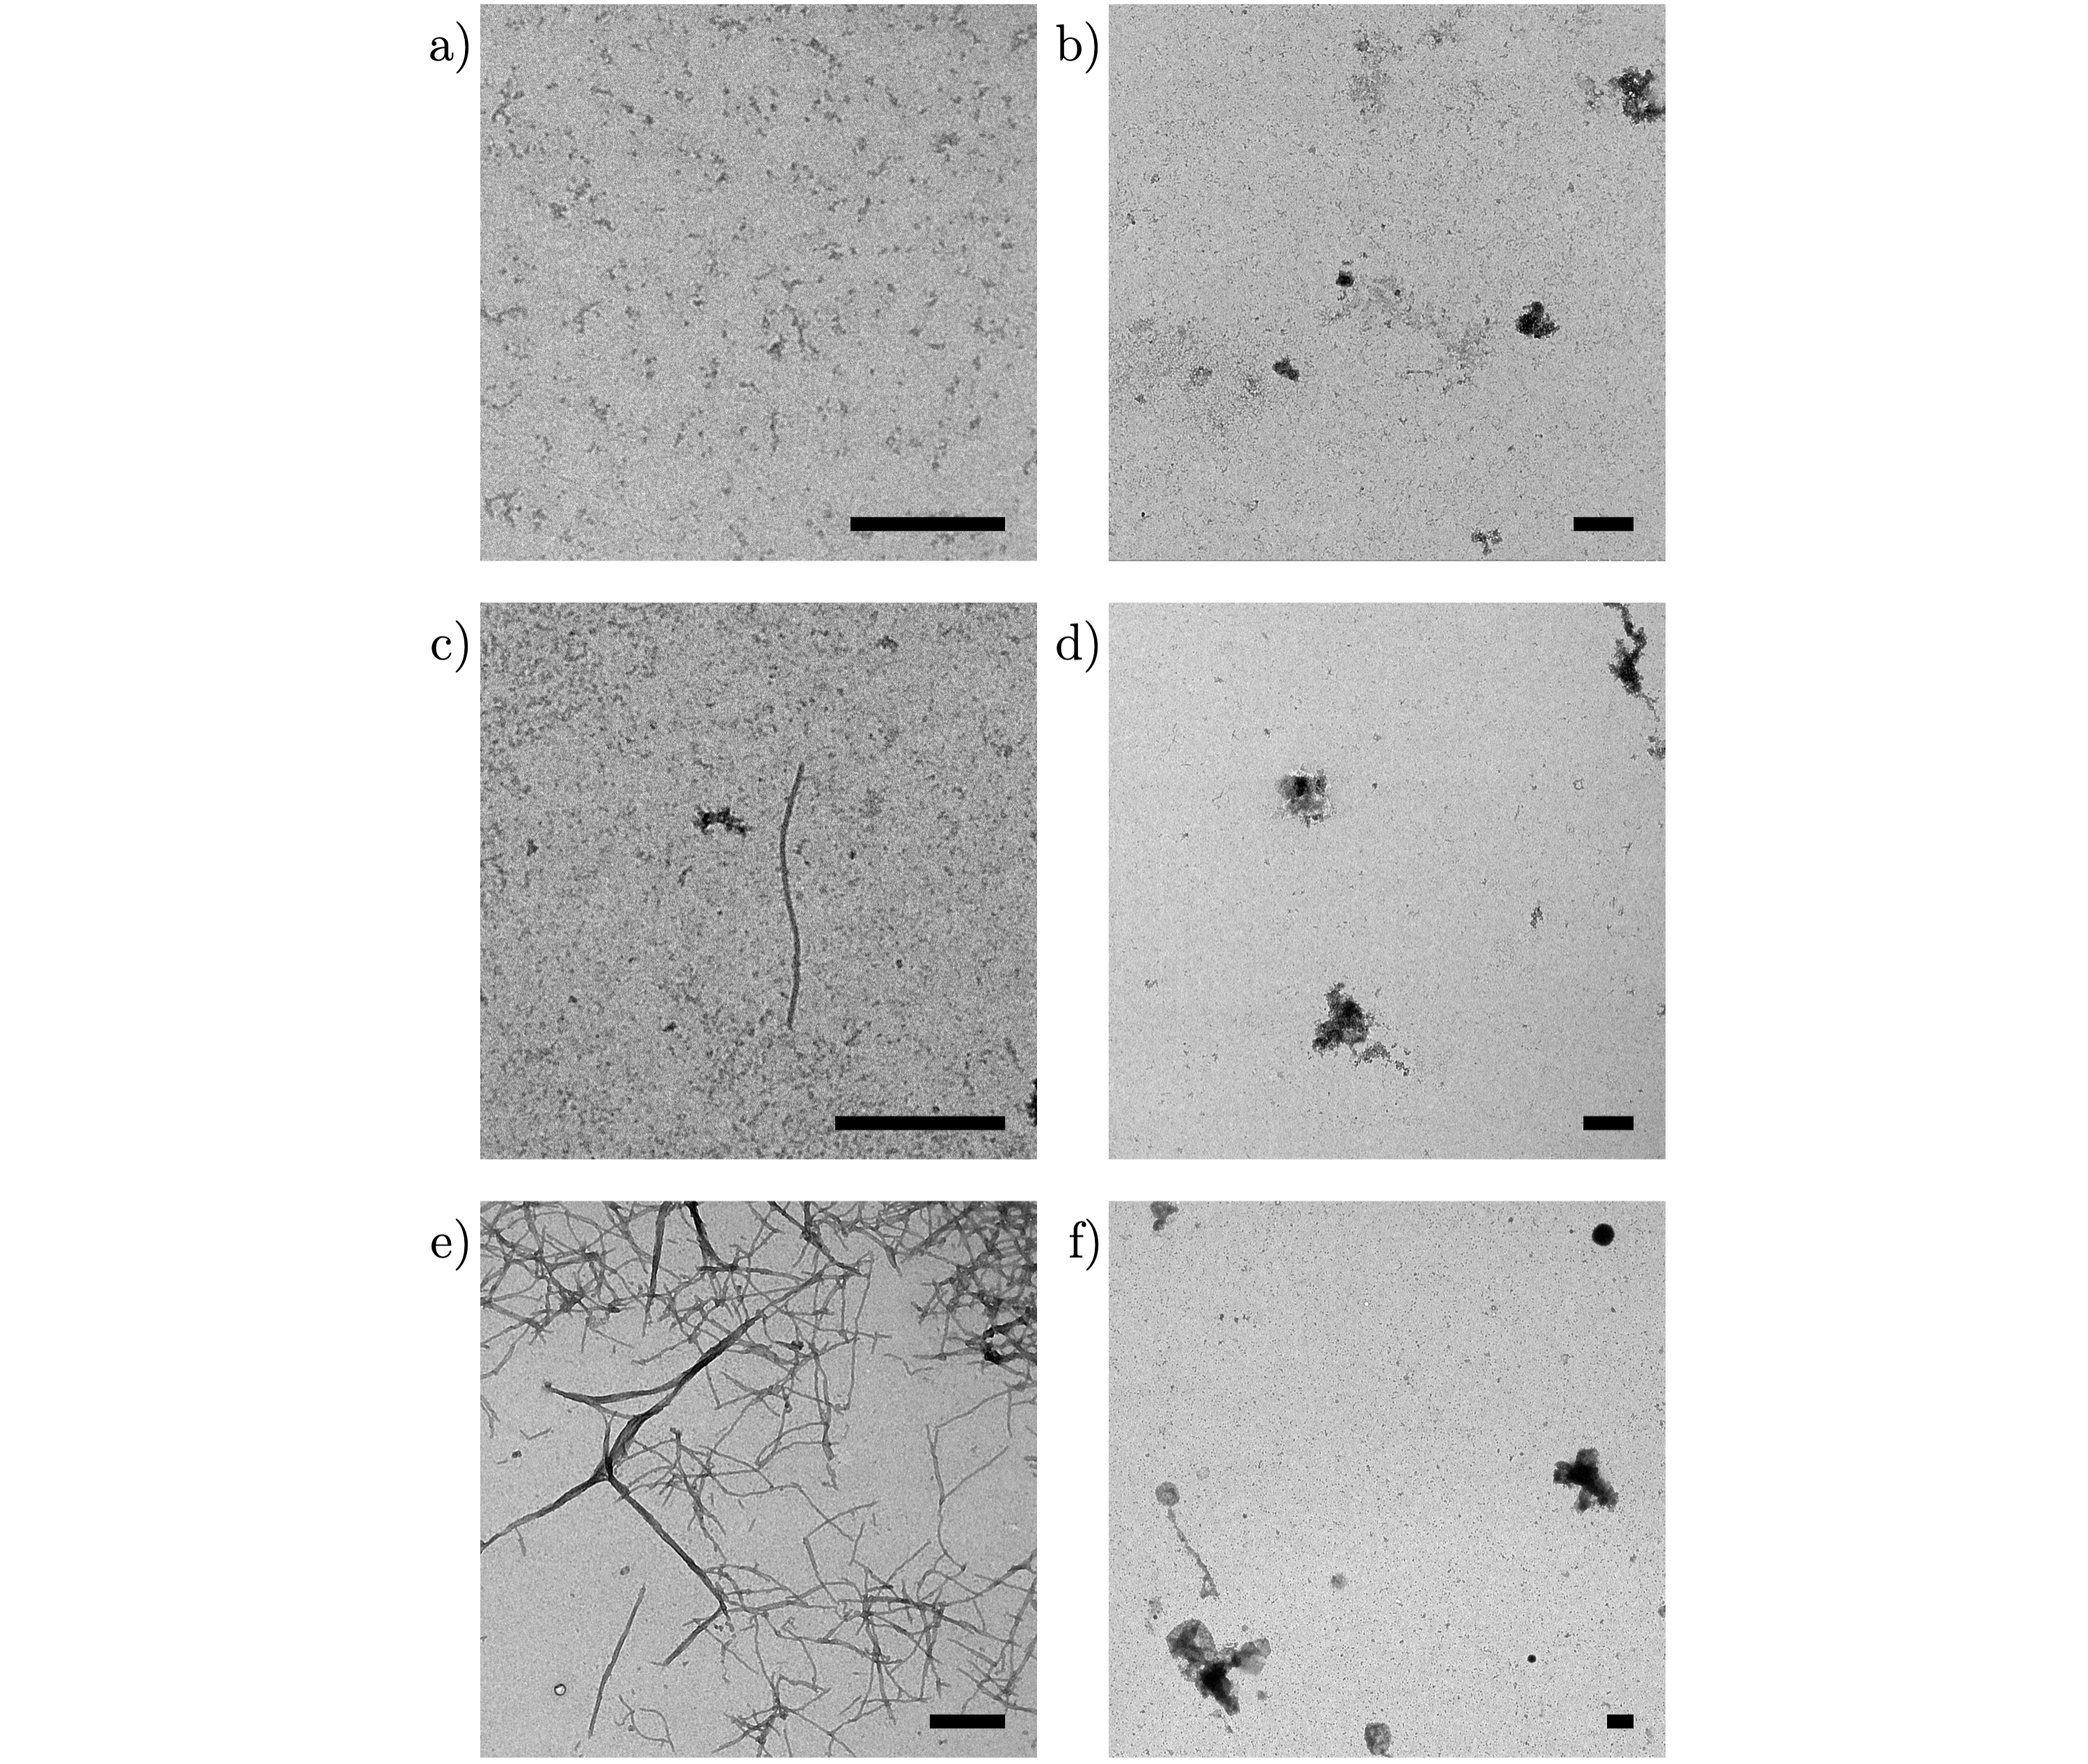
\includegraphics{lab/em_overview.png}
\caption{\textbf{TEM images of samples following CaptoCore purification. } Images are shown for the constructs d29-A (a), S-Tag-A (b), S-Tag-B (c), PVX CP (d), a control sample of S-Tag PVX virions (e), and a sample from ALiCE reaction mix using a non-template, captured using the anti-PVX antibody (f). The image for the non-template sample was provided by the Institute of Molecular Biotechnology. The black bars mark a length of \SI{500}{\nano\meter}. The control sample shows a network of flexible, filamentous particles. The sample from S-Tag-A showed two rod-like structures over all images. Other samples did not contain signs of tubular particles. }
\label{fig:em_overview}
\end{figure}

The images for S-Tag-B were similar in appearance to those of the non-template control, but included two rod-like structures, one of which appeared flexible with a diameter of ~\SI{15}{\nano\meter} (~\SI{760}{\nano\meter} length), and the other appearing more rigid with a diameter of ~\SI{24}{\nano\meter} (~\SI{850}{\nano\meter} length) (\autoref{fig:em_particles}). 

\begin{figure}
\includegraphics{lab/em_particles.png}
\caption{\textbf{TEM images of rod-like structures in the sample of the design S-Tag-B. } The two shown images display the only tubular structures found in the sample. The structure in (a) appears flexible with a diameter of ~\SI{15}{\nano\meter} and a length of ~\SI{760}{\nano\meter}, while the structure in (b) appears more rigid with a diameter of ~\SI{24}{\nano\meter} and a length of ~\SI{850}{\nano\meter}.}
\label{fig:em_particles}
\end{figure}
